\begin{frame}
  \frametitle{Code Coverage}
  {\Large\color{Base09}What percentage of our source code has been executed by our tests?}
  \begin{block}{Procedure}
  \begin{itemize}
  \item Compile/link with coverage flags.
  \item Run all tests.
  \item Generate readable statistics with one of:
    \begin{itemize}
    \item gcov
    \item lcov
    \end{itemize}
  \item Optionally run genhtml to produce visually pleasant version.
  \end{itemize}
  \end{block}
\end{frame}

\begin{frame}[fragile]
  \frametitle{Code Coverage}
  \begin{example}
    \begin{lstlisting}[style=C]
  int to_test( int x )
  {
    int ii;
    int sum = 0;
    for( ii = 0; ii < 10; ++ii )
    {
      if( x == 0 )
        sum += ii;
      else if( x == 1 )
        sum += 2*ii;
      else
        sum += 3*ii;
    }
    return sum;
  }
    \end{lstlisting}
  \end{example}
\end{frame}

\begin{frame}[fragile]
  \frametitle{Code Coverage}
  \begin{block}{Compile with coverage}
    \vspace{0.2cm}
    \hspace{0.2cm}{\ttfamily gcc -g -O0 {\color{Base09}-fprofile-arcs -ftest-coverage} in.c}
    \vspace{0.2cm}
  \end{block}
  \begin{block}{Run to generate stats}
    \vspace{0.2cm}
    \hspace{0.2cm}{\ttfamily ./a.out}

    \vspace{0.2cm}
    \hspace{1cm} or, more likely,
    \vspace{0.2cm}

    \hspace{0.2cm}{\ttfamily make check}
    \vspace{0.2cm}
  \end{block}
\end{frame}

\begin{frame}[fragile]
  \frametitle{Code Coverage}
  \begin{block}{Run lcov}
    \vspace{0.2cm}
    \hspace{0.2cm}{\ttfamily lcov -c --directory . --output-file results.info}
    \vspace{0.2cm}
  \end{block}
  \vspace{1cm}
  \begin{block}{Generate HTML}
    \vspace{0.2cm}
    \hspace{0.2cm}{\ttfamily genhtml results.info --output-directory html}
    \vspace{0.2cm}
  \end{block}
\end{frame}

\begin{frame}
  \frametitle{Code Coverage}
  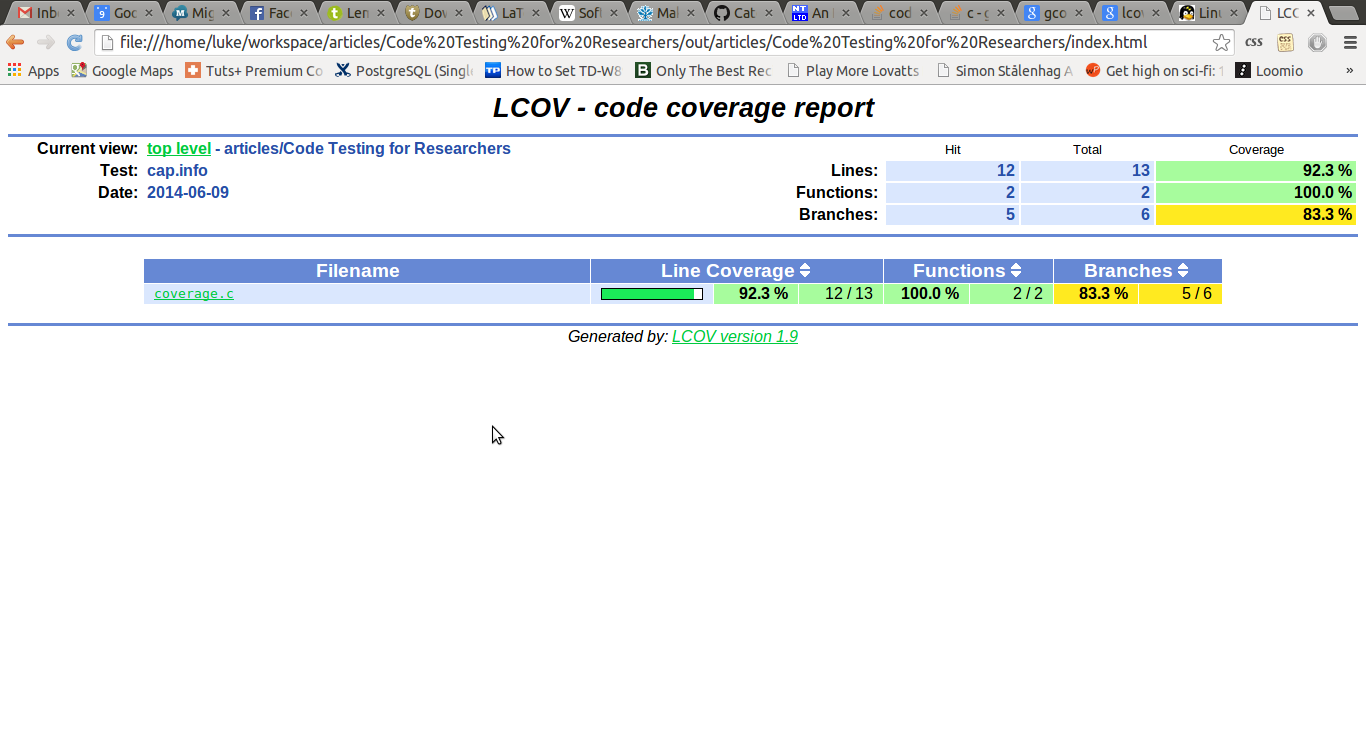
\includegraphics[width=\textwidth]{gcov-1.png}
\end{frame}

\begin{frame}
  \frametitle{Code Coverage}
  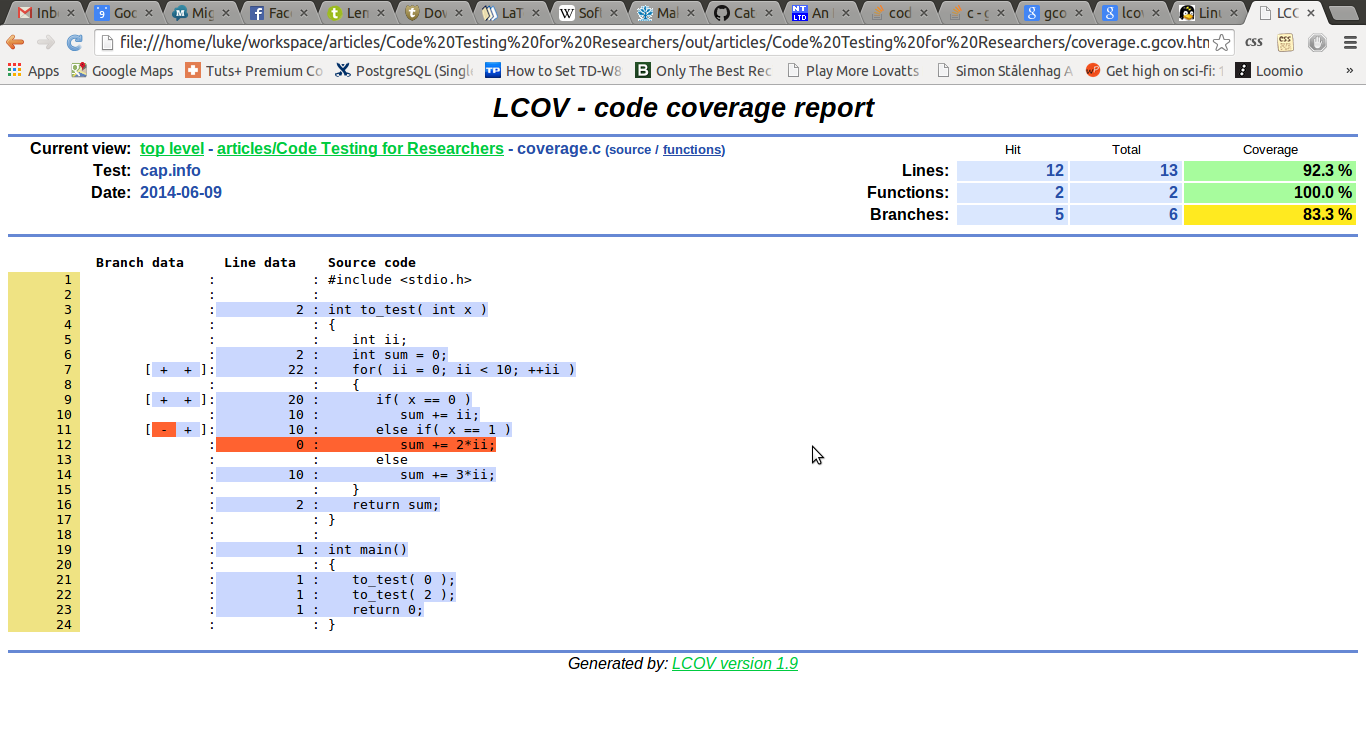
\includegraphics[width=\textwidth]{gcov-2.png}
\end{frame}
